\documentclass[12pt, a4paper, twoside]{article}
\usepackage{labreport}
\usepackage{pdfpages}

\setlabreportopts[authors={Nandor Kovacs \& Céline Schuster},
    title={Mathematisches Pendel},
    subtitle={Untersuchung der Eigenschaften eines Mathematischen Pendels},
    date={\today},
    labdate={10. März 2022}
]

\begin{document}
\maketitlepage

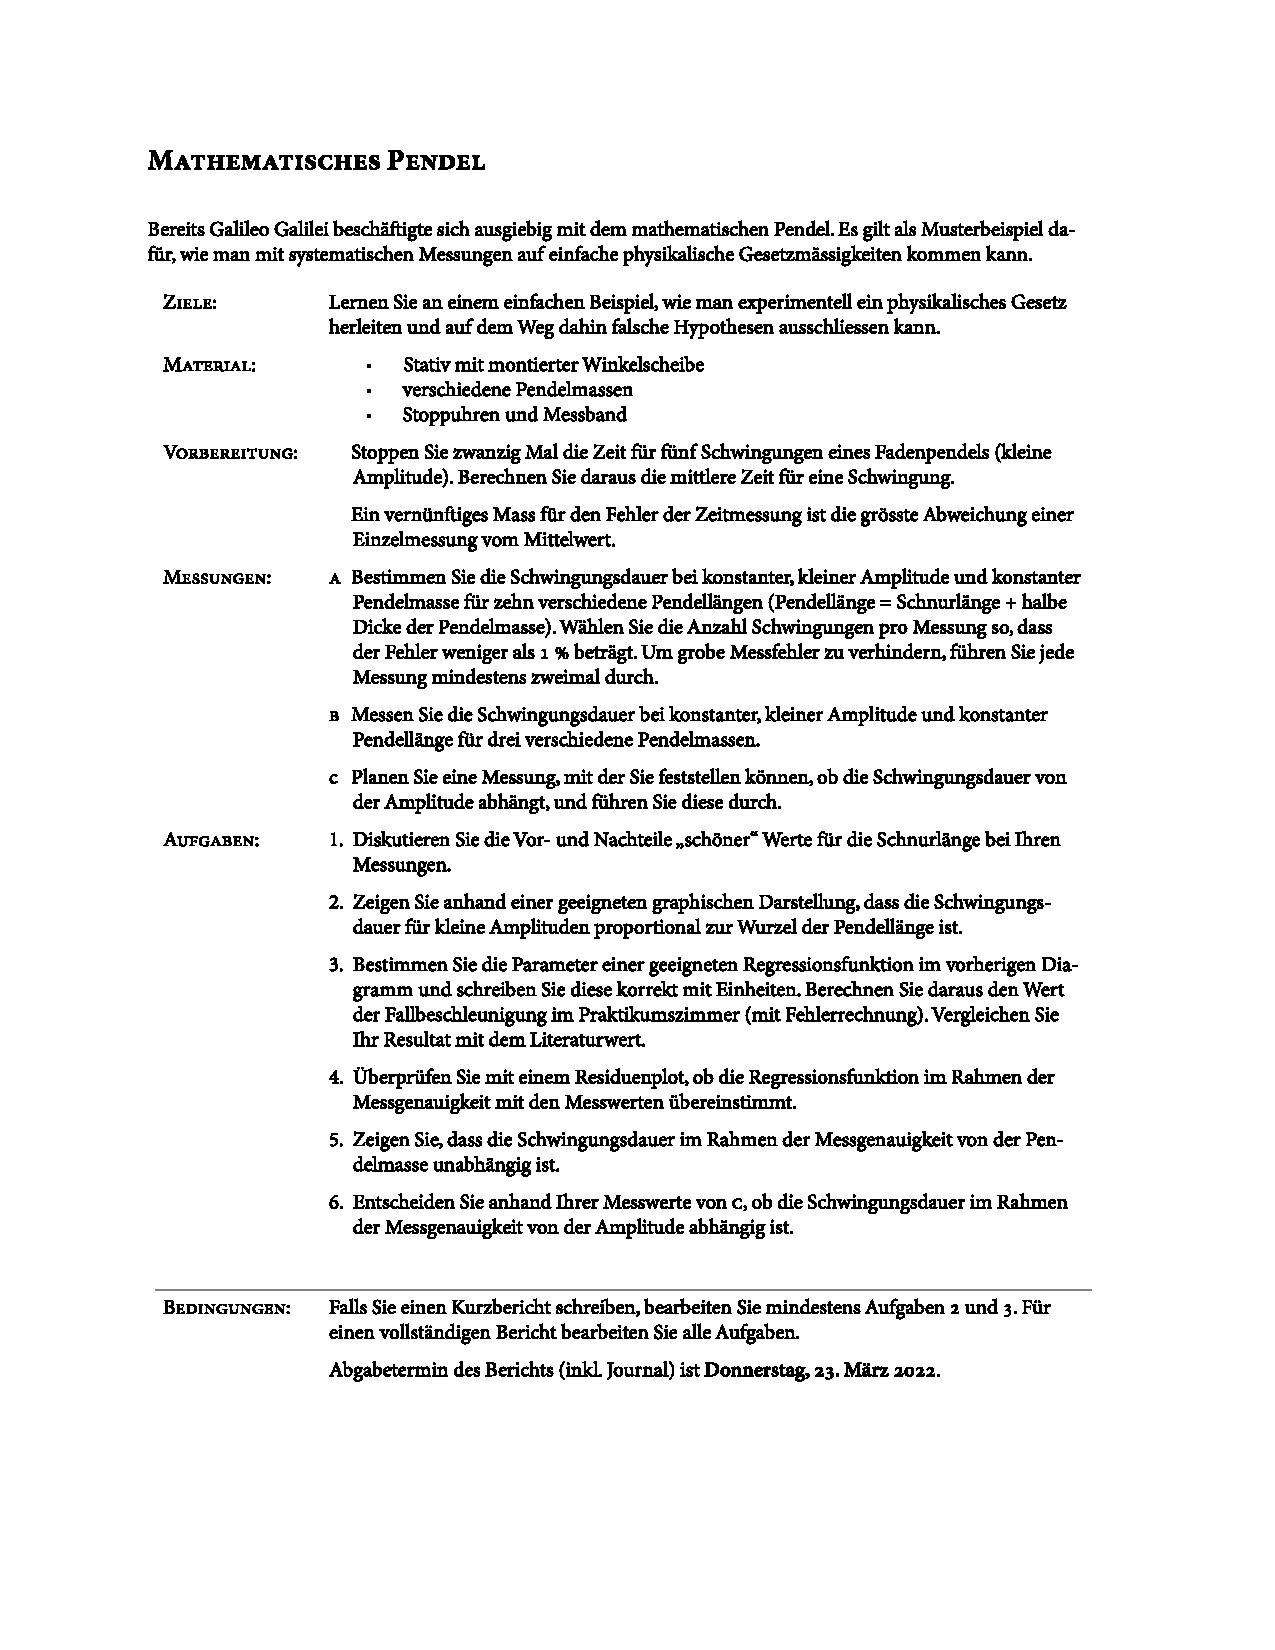
\includepdf[pages={1}]{aufgabenstellung.pdf}

\section{Einleitung}
Wir alle kennen Pendeluhren.
Pendeluhren benutzen statt Quartzstückchen oder Signale von einer Radiouhr eine Pendel, um die Zeit zu verfolgen.
Das muss heissen, dass die Periodenlängen von Pendeln berechenbar sind.
Falls die Periode von dem Ausschlagwinkel abhängt, würde das aber recht kompliziert sein zum berechnen, also vermuten wir dass beispielsweise das nicht der Fall ist.

\section{Theorie}
Eine Pendel hat folgende Parameter:
\begin{list}{-}{}
  \item $l$ = die Länge der Pendel
  \item $g$ = das Gewicht des Pendelgewichts. Dies ist gleich zu der Länge der Schnur plus die halbe Dicke des Gewichts.
  \item $\alpha$ = die Auslenkung beim starten der Pendel in Winkelgrade.
\end{list}

Die Formel für die länge einer Periode in Sekunden lautet:
$$T=2\pi \sqrt{\frac{l}{g}}$$
\cite{FoTa}

\section{Experiment}
\begin{figure} [ht]
  \centering
  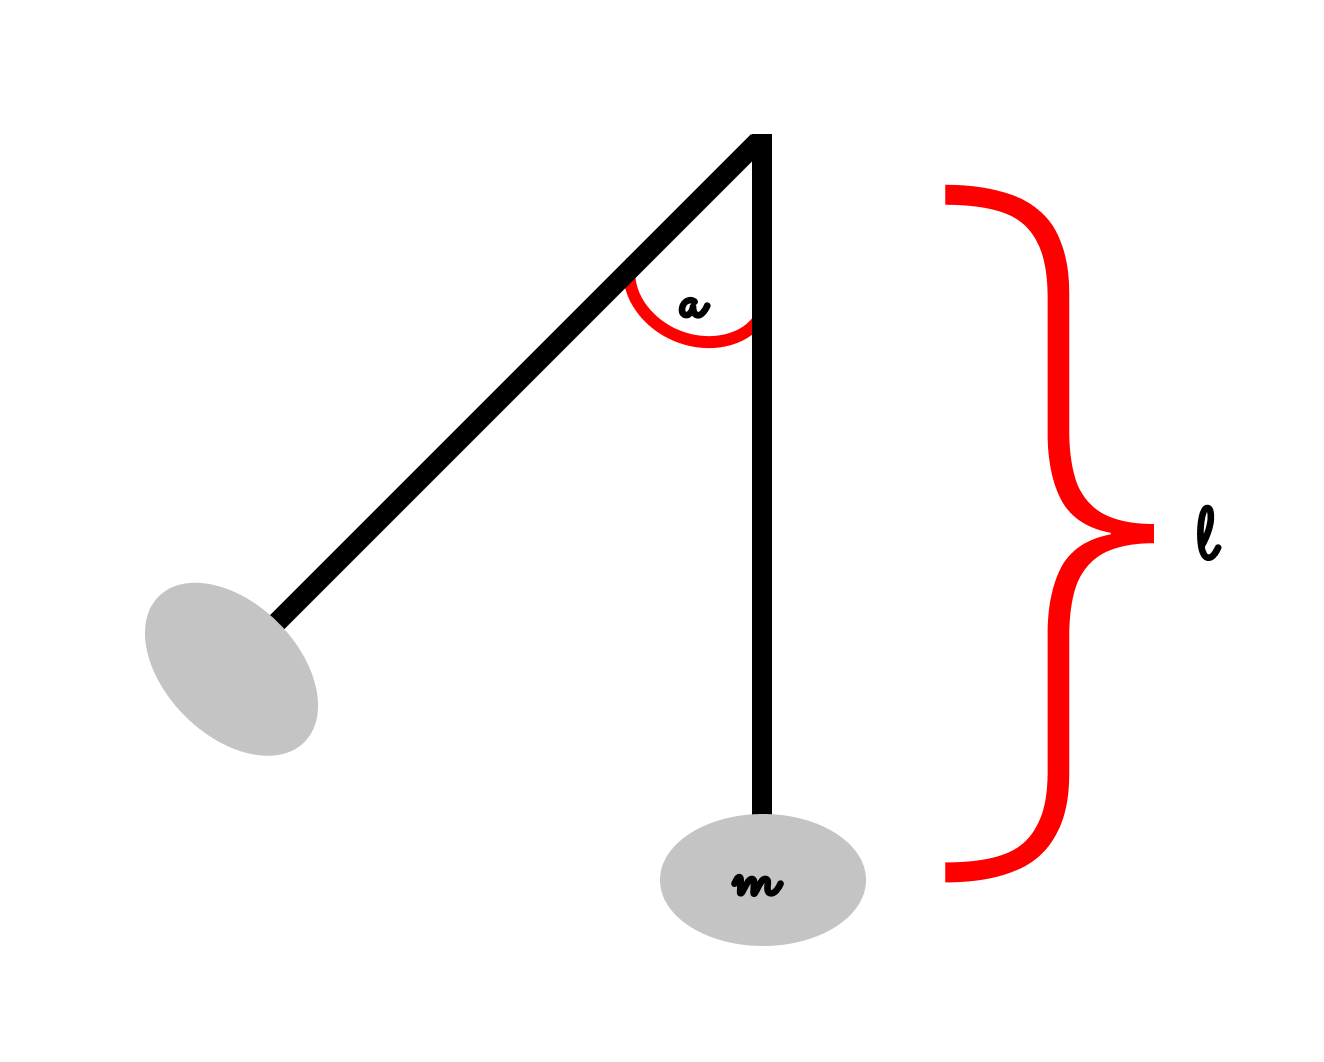
\includegraphics[width=0.5\textwidth]{Experimentaufbau.png}
  \caption{Skizze Experimentaufbau}
  \label{fig:experimentaufbau}
\end{figure}

Unser Experiment ist einfach aufgebaut.
Es wird ein Gewicht an einem Faden Aufgehängt.
Sie wird ausgelenkt, losgelassen, und es wird die Zeit gemessen, die die Pendel für 5 Perioden braucht.
Wir starten die Messung wenn die Pendel die Mitte kreuzt, und Enden sie wenn sie 5mal hin und her ist. So werden wir 5mal so prezise sein.

Die Länge $l$ messen wir mit einem Massband auf 0.5cm genau und $\alpha$ messen wir mit einer Winklerscheibe auf 2\textdegree genau.
Die Masse $m$ messen wir mit einer Waage auf 0.1g genau.
Die Zeit messen wir mit einer Stoppuhr. Damit wir genauere Messungen haben, messen wir immer 5 Perioden.

Um die genauigkeit von den Zeitmessungen zu bestimmen, messen wir 20mal mit dem gleichen $\alpha$, $m$, und $l$.
Wir berechnen die maximale Abweichung mit diesen Daten.

\datatable{2}{Messungen zur Vorbereitung}{Nr. & Periodenlänge $T$*5 in s}{precision.csv}{precision}


\begin{align*}
  \overline{T_5} & = \frac{1}{n} \sum_{i=1}^{n} T_{i}=\frac{1}{n}\left(T_{1}+\cdots+T_{n}\right) \\
                 & =\frac{164.01s}{20}                                                           \\
                 & =8.2005s                                                                      \\
  \\
  \Delta T_5     & = max(T_{max} - \overline{T}, \overline{T} - T_{min})                         \\
                 & = max(8.27s - 8.2005s, 8.2005s - 8.14)                                        \\
                 & = max(0.0695s, 0.0605)                                                        \\
                 & = 0.0695s                                                                     \\
                 & = 0.07s                                                                       \\
  \Delta T       & = \Delta T_5 / 5                                                              \\
                 & =0.014                                                                        \\
\end{align*}

Da die Zeitmessung 5 Periodenlängen entspricht, ist die genauigkeit dementsprechend auch 5mal so gut.
Das heisst, das $T$ auf $0.014$ genau gemessen ist.
Die Stoppuhr zeigt $0.01$ genau an, was bei 5 Schwingungen einer Genauigkeit von $0.002$ entsprechen würde.
Die Stoppuhr ist also genauer wie unsere Messkünste, und darum nehmen wir den $\Delta T$ von unseren Messkünsten als absoluten Fehler.

\section{Messungen}
\datatable{2}{$m$ ist konstant, $\alpha$ ist konstant und klein, $l$ ist variabel}{Pendellänge $l$ in cm & Periodenlänge $T$*5 in s}{laenge.csv}{laenge}
\datatable{2}{$l$ ist konstant, $\alpha$ ist konstant und klein, $m$ ist variabel}{Gewichtsmasse $m$ in g & Periodenlänge $T$*5 in s}{masse.csv}{masse}
\datatable{2}{$l$ ist konstant, $m$ ist konstant, $\alpha$ ist variabel}{Amplitude $\alpha$ in Winkelgrad & Periodenlänge $T$*5 in s}{winkelgrad.csv}{winkel}

\section{Aufgaben}
\subsection{Vor und Nachteile schöner Werte für $l$}
Schöne Längen für $l$ sind einfacher zu messen, was ein deutlicher Vorteil ist.
Das Problem ist, das wenn $l$ einen schönen Wert hat, dann wird $T$ relativ sicher keinen schönen Wert haben.

\subsection{Proportionalität von $T$ zu $l$}

\begin{center}
  \pgfplotsset{every axis legend/.append style={
        at={(1,0)},
        anchor=south east}}
  \begin{tikzpicture}
    \begin{axis}[
        xmin=-0.2,
        xmax=2,
        ymin=0,
        ymax=2.2,
        axis lines = left,
        % enlargelimits=0.2,
        ylabel={Periodenlänge $T$ in s},
        xlabel={Pendellänge $l$ in m},
        cycle list name=black white
      ]
      \addplot+[color=red, samples=1000, mark=none]{sqrt(x)};
      \addlegendentry{sqrt(x)}
      \addplot+[only marks] plot [error bars/.cd, y dir=both, x dir=both, x fixed=0.001, y fixed=0.014] table[x expr=\thisrow{l} / 100, y expr=\thisrow{T} / 5, col sep=comma] {laenge.csv};
      \addlegendentry{unsere messungen}
    \end{axis}
  \end{tikzpicture}
\end{center}


Diese Grafik illustriert gut das $T$ proportional zur Wurzel von $l$ ist.
Die Fehlerbalken sind so klein, dass sie nicht sichtbar sind.

\subsection{Regressionsfunktion \& Fallbeschleunigung ausrechnen}
\subsubsection{Regressionsparameter berechnen}
Der Regressionsfaktor $R_l$ ist:

\begin{align*}
  R_l & = \frac{sqrt(l)}{T_l} \\
\end{align*}

Um eine Annäherung an der allgemeinen Regressionsfaktor zu bekommen,
nehmen wir den Druchschnitt aller $R_l$ die wir ausrechnen können aus unseren Messresultaten aus Tabelle~\ref{table:laenge}:

\begin{align*}
  \overline{R} & = \frac{1}{n}\sum_{i=0}^{n} \frac{sqrt(l_i)}{T_i} \\
  \\
               & = \frac{9.923360844s}{20\sqrt{m}}                 \\
  \\
               & = 0.496168042\frac{s}{sqrt(m)}
\end{align*}

Der Literarturwert für $R$ kann man aus dem Literarturwert für $T$ ausrechnen:

\begin{align*}
  T                             & = 2\pi \sqrt{\frac{l}{g}}    \\
  \frac{\sqrt{g}}{2\pi}T        & = \sqrt{l}                   \\
  \\
  R                             & = \frac{\sqrt{g}}{2\pi}      \\
  \\
  \frac{\sqrt{9.81m/s^2}}{2\pi} & = 0.498488\frac{\sqrt{m}}{s} \\
\end{align*}

\subsubsection{Fallbeschleunigung mit Fehlerrechnung ausrechnen}
Nehmen wir an das der Wert für $R$ den wir berechnet haben korrekt ist.
Das würde heissen, das $R = 0.496168042\frac{\sqrt{m}}{s}$

\begin{align*}
  \frac{\sqrt{g}}{2\pi} & = 0.496168042\frac{\sqrt{m}}{s}           \\
  \sqrt{g}              & = 2\pi\cdot 0.496168042\frac{\sqrt{m}}{s} \\
  g                     & = (2\pi\cdot0.496168042)^2\frac{m}{s^2}   \\
  g                     & = 9.7189\frac{m}{s^2}                     \\
\end{align*}

Laut unserem $R$ Wert würde $g$ 9.7182 entsprechen. Fehlerquellen sind die ungenauen Messungen.
$T$ ist auf $0.014$ genau angegeben, und l auf $0.001$ genau angegeben.
Das heisst:
\begin{align*}
  \Delta T & = 0.014s \\
  \Delta l & = 0.001m \\
\end{align*}

Der relative Fehler ändert sich. Hier nehmen wir wieder den Druchschnitt aller relativer Fehler.

\begin{align*}
  \Delta r_T & = \frac{1}{n}\sum_{i=0}^{n}\frac{\Delta r_T}{T_i} \\
             & = \frac{0.22}{20}                                 \\
             & = 0.011                                           \\
  \\
  \Delta r_l & = \frac{1}{n}\sum_{i=0}^{n}\frac{\Delta r_l}{l_i} \\
             & = \frac{0.059}{20}                                \\
             & = 0.0295                                          \\
  \\
\end{align*}

Jetzt wo wir alle relative und absolute Messfehler kennen, können wir die restlichen Fehler berechnen:

\begin{align*}
  R          & = \frac{sqrt(l)}{T}                           \\
  \Delta r_R & = \Delta r_l\frac{1}{2}+\Delta r_T            \\
             & = 0.0295\frac{1}{2} + 0.011                   \\
             & = 0.02572                                     \\
  \\
  g          & = (2\pi\cdot R)^2                             \\
  \Delta r_g & = 2\Delta R                                   \\
             & = 0.05144                                     \\
  \Delta g   & = g * \Delta r_g                              \\
             & = 9.7189\frac{m}{s^2} * 0.05144               \\
             & = 0.49994\frac{m}{s^2} \approx 0.5\frac{m}{s^2} \\
\end{align*}                     

Das heisst, das $g = 9.7189\frac{m}{s^2} \pm 0.5\frac{m}{s^2}$

\subsection{Residuenplot}

\begin{center}
  \pgfplotsset{every axis legend/.append style={
        at={(1,0)},
        anchor=south east}}
  \begin{tikzpicture}
    \begin{axis}[
        xmin=-0.2,
        xmax=2,
        ymin=0,
        ymax=2.2,
        axis lines = left,
        % enlargelimits=0.2,
        ylabel={Periodenlänge $T$ in s},
        xlabel={Pendellänge $l$ in m},
        cycle list name=black white
      ]
      \addplot+[color=red, samples=1000, mark=none]{sqrt(x)};
      \addlegendentry{sqrt(x)}
      \addplot+[only marks] plot [error bars/.cd, y dir=both, x dir=both, x fixed=0.001, y fixed=0.014] table[x expr=\thisrow{l} / 100, y expr=\thisrow{T} / 5 * 0.496168042, col sep=comma] {laenge.csv};
      \addlegendentry{unsere messungen * $\overline{R}$}
    \end{axis}
  \end{tikzpicture}
\end{center}

\begin{center}
  \pgfplotsset{every axis legend/.append style={
        at={(1,1)},
        anchor=north east}}
  \begin{tikzpicture}
    \begin{axis}[
        xmin=-0.2,
        xmax=0.5,
        ymin=0,
        ymax=2.2,
        axis lines = left,
        % enlargelimits=0.2,
        ylabel={Periodenlänge $T$ in s},
        xlabel={Pendellänge $l$ in m},
        cycle list name=black white
      ]
      \addplot+[color=red, samples=1000, mark=none]{sqrt(x)};
      \addlegendentry{sqrt(x)}
      \addplot+[only marks] plot [error bars/.cd, y dir=both, x dir=both, x fixed=0.001, y fixed=0.014] table[x expr=\thisrow{l} / 100, y expr=\thisrow{T} / 5 * 0.496168042, col sep=comma] {laenge.csv};
      \addlegendentry{unsere messungen * $\overline{R}$}
    \end{axis}
  \end{tikzpicture}
\end{center}

Anhand von diesen Residuenplots sehen wir,
dass unser Wert für $R$ der sehr gut der Messgenauigkeit entspricht.
Die Fehlerbalken sind so klein, dass man sie nicht einmal sieht beim vergrösserten Plot.

\subsection{Einfluss der Pendelmasse}
\begin{center}
  \pgfplotsset{every axis legend/.append style={
        at={(1,1)},
        anchor=north east}}
  \begin{tikzpicture}
    \begin{axis}[
        axis lines = left,
        enlargelimits=0.2,
        ylabel={Periodenlänge $T$ in s},
        xlabel={Gewichtsmasse $m$ in g},
        cycle list name=black white
      ]

      \addplot+[only marks] plot [error bars/.cd, y dir=both, x dir=both, x fixed=0.1, y fixed=0.014] table[x expr=\thisrow{m}, y expr=\thisrow{T} / 5, col sep=comma] {masse.csv};
      \addlegendentry{unsere messungen}
      \addplot+[mark=none, color=red, samples=4, domain=0:400] {1.0133};
      \addlegendentry{durchschnitt der messungen}
    \end{axis}
  \end{tikzpicture}
\end{center}

Alle Messwerte sind innerhalb von den Fehlerbalken von allen anderen Messwerten.
$T$ ist unabhängig von $m$ innerhalb von der Messgenauigkeit.

\subsection{Einfluss der Amplitude}
\begin{center}
  \pgfplotsset{every axis legend/.append style={
        at={(1,1)},
        anchor=north east}}
  \begin{tikzpicture}
    \begin{axis}[
        axis lines = left,
        enlargelimits=0.2,
        ylabel={Periodenlänge $T$ in s},
        xlabel={Amplitude $\alpha$ in winkelgrad},
        cycle list name=black white
      ]
      \addplot+[only marks] plot [error bars/.cd, y dir=both, x dir=both, x fixed=0.1, y fixed=0.014] table[x expr=\thisrow{f}, y expr=\thisrow{T} / 5, col sep=comma] {winkelgrad.csv};
      \addlegendentry{unsere messungen}
      \addplot+[mark=none, color=red, samples=4, domain=0:35] {8.48833/5};
      \addlegendentry{durchschnitt der messungen}
    \end{axis}
  \end{tikzpicture}
\end{center}

Alle Messwerte sind innerhalb von den Fehlerbalken von allen anderen Messwerten.
$T$ ist unabhängig von $\alpha$ innerhalb von der Messgenauigkeit.
\section{Fazit}
Wir können innerhalb von unserer Messgenauigkeit bestätigen das nur die Länge der Pendel die Periodenlänge beeinflusst hier auf der Erde.
\par
Ausserdem konnte ($\Delta g_{relativ} = 0.05144$) $g$ mit einer relativ grossen Genauigkeit ausgerechnet werden.

\section{Reflektion}
Wir haben in diesem Physikpraktikum gelernt wie man Messungen macht, und dessen Fehlerquoten dokumentiert und berrechnet.
Ausserdem haben gelernt wie man einen Bericht über Messwerte schreibt.

Wir hatten eine kleine Fehlkomunikation was die Messtechnik anging, was dazu führte das alle unsere Werte halb so gross waren.
Unsere Fehlerrechnung scheint gut zu sein, aber der Fehler den wir Bekommen haben ist etwas zu klein.
\section{Anhang}
Versuchsanleitung und Originalprotokoll vom \labdate

\end{document}
